\section{The Identity-Transformation Approach}
\label{sec:challenge}

In this section,
    we firstly list the security requirements of SSO,
        and present the identity-transformation approach.

\subsection{Security Requirements for SSO Services}
\label{subsec:basicrequirements}

Non-anonymous SSO services are designed to allow a user to log into an honest RP as her unique account at this RP, %correlating multiple logins,
by presenting identity tokens issued by a trusted IdP   \cite{OpenIDConnect,rfc6749,SAML,SAMLIdentifier,NIST2017draft}.
%It makes no sense to discuss the login results at a malicious RP. 
This security goal is achieved through the following properties of identity tokens.

First of all, \emph{authenticity}, \emph{confidentiality}, and \emph{integrity} of identity tokens are necessary to prevent forging, eavesdropping and tampering.
In SSO services, identity tokens are issued by the trusted IdP,
    transmitted over HTTPS/TLS \cite{OpenIDConnect, rfc6749, SAML},
    and finally forwarded to the target RPs by the authenticated user.
Common security mechanisms within a browser (e.g., the mechanisms of HTTP session and \verb+postMessage+ targetOrigin)
are also required for confidentiality of tokens \cite{GoogleIdIntegrate,de2014oauth,FettKS14,BrowserID} (see Section \ref{sec:web-design} for details).

Meanwhile, in each login the IdP issues an identity token that (\emph{a}) specifies the target RP (i.e., \emph{RP designation}) and (\emph{b}) identifies the authenticated user who requests this token (i.e., \emph{user identification}),
        as the enclosed (pseudo-)identities of RP and user \cite{OpenIDConnect,rfc6749,SAML} (see Section \ref{analysis-security} for details).
RP designation prevents malicious RPs from replaying received identity tokens to gain illegal access to other honest RPs as victim users.
So an RP usually checks the RP (pseudo-)identity enclosed in a token before accepting it 
\cite{OpenIDConnect,BrowserID,SPRESSO,NIST2017draft,POIDC,save-flow,up-sso,miso}
 and then allows the token holder to log in as the specified (pseudo-)identity (i.e., account).

%The requirements for secure SSO services, i.e., RP designation, user identification, integrity, and confidentiality of identity tokens, have been extensively studied \cite{ArmandoCCCT08, SPRESSO, FettKS14, FettKS16, FettKS17}.
%Any vulnerabilities that undermine these properties result in various attacks \cite{SomorovskyMSKJ12, WangCW12, ArmandoCCCPS13, ZhouE14, WangZLLYLG15, WangZLG16, YangLLZH16, MainkaMS16, MainkaMSW17, YangLCZ18, YangLS17, ShiWL19, ChenPCTKT14, ccsSunB12, DiscoveringJCS, dimvaLiM16, CaoSBKVC14, TowardsShehabM14}.

\subsection{Identity Transformations in SSO}
\label{subsec:solutions}

%As mentioned above, in order to ensure, the visited RP and the authenticated user are specified in an identity token as their identities or pseudo-identities.

As analyzed in Section \ref{subsec-solutions},
    existing privacy-preserving solutions of SSO hide only RP identities or user identities
    (i.e., only IdP-based login tracing or RP-based identity linkage is prevented),
        or introduce an extra fully-trusted server to process the (pseudo-)identities of both RP and user before an identity token is issued.
       % \footnote{In privacy-preserving identity federation, a user by herself keeps a long-term secret to mask the relationship of these (pseudo-)identities and accounts.}

UPPRESSO attempts to \emph{simultaneously} transform the identities of RP and user in each login,
        without extra trusted servers more than the honest-but-curious IdP,
         to provide untraceable and unlinkable SSO service.
%
%Therefore, we try to implement privacy-preserving SSO that ensures security as above, while preventing both IdP-based login tracing and RP-based identity linkage.
%The requirements of security and privacy are satisfied through \emph{transformed identities} in the identity tokens.
Table \ref{tbl:notations-dilemma} lists the notations of the identity-transformation approach,
and a sub/super-script (i.e., $i$, $j$, or $l$) may be omitted if it does not cause ambiguity.

\begin{table}[t]
\footnotesize
    \caption{The (pseudo-)identities in the identity transformations}
    \centering
%    \begin{tabular}{|l|l|l|}
    \begin{tabular}{|l|p{5.15cm}|l|} \hline
    {\textbf{Notation}} & {\textbf{Definition}} & {\textbf{Lifecycle}} \\ \hline
    {$ID_{U_i}$} & {The $i$-th user's unique identity at the IdP.} & {Permanent} \\ \hline
    {$ID_{RP_j}$} & {The $j$-th RP's unique identity at the IdP.} & {Permanent} \\ \hline
    {$Acct_{i,j}$} & {The $i$-th user's account at the $j$-th RP.} & {Permanent} \\ \hline
    {$PID_{U_i,j}^l$} & {The $i$-th user's pseudo-identity in her $l$-th login visiting the $j$-th RP.} & {Ephemeral} \\ \hline
    {$PID_{RP_j}^l$} & {The $j$-th RP's pseudo-identity in the user's $l$-th login visiting this RP.} & {Ephemeral} \\ \hline
    \end{tabular}
    \label{tbl:notations-dilemma}
\end{table}


%Since an IdP authenticates users and always knows the user's identity (i.e., $ID_U$),
%    to prevent IdP-based login tracing, we should not reveal the target RP's identity (i.e., $ID_{RP}$) to the IdP.
%So an ephemeral pseudo-identity for the RP (i.e., $PID_{RP}$) should be used in the identity-token request: (\emph{a}) to ensure RP designation, ephemeral $PID_{RP}$ should be uniquely associated with the target RP;
% and (\emph{b}) the IdP cannot derive any information about IDRP from any PIDi RP, which implies PIDi RP in multiple logins should be independent of each other.

%While RP designation and user identification are required to ensure security of SSO services,
%    we present the identity-transformation approach to provide privacy guarantees.


First of all, each user owns her account unique at an RP.
$\mathcal{F}_{Acct\ast}(ID_{U_i}, ID_{RP_j}) = Acct_{i,j}$ is proposed to determine a user's account at an RP.
An account belonging to some user is \emph{meaningful},
while a \emph{meaningless} account at an RP does not belong to any user.

To ensure IdP untraceability (or prevent IdP-based login tracing),
    a user initiates a login by calculating an \emph{ephemeral} pseudo-identity $PID^l_{RP_j}$  for the target RP and sending an identity-token request for $PID^l_{RP_j}$ (but not $ID_{RP_j}$) to an IdP.

After authenticating the initiating user as $ID_{U_i}$, the IdP calculates an \emph{ephemeral} $PID^l_{U_i,j}$ based on $ID_{U_i}$ and $PID^l_{RP_j}$, and then issues an identity token that binds $PID^l_{U_i,j}$ and $PID^l_{RP_j}$.
To ensure RP unlinkability (or prevent RP-based identity linkage),
    $ID_{U_i}$ is not enclosed in the identity token.
%Meanwhile, the calculation of $PID_U$ involves $ID_U$, and then the user is identified implicitly.

On receiving a signed token, the RP calculates the user's \emph{permanent} account (i.e., $Acct_{i,j}$) based on $PID^l_{U_i,j}$ and $PID^l_{RP_j}$,
and allows the token holder to log in as $Acct_{i,j}$.

Therefore, in addition to $\mathcal{F}_{Acct\ast}(ID_{U}, ID_{RP}) = Acct$,
we propose the following identity transformations in a login initiated by a user to visit an RP in privacy-preserving SSO:
\begin{itemize}
\setlength{\topsep}{0pt}
\setlength{\partopsep}{0pt}
\setlength{\itemsep}{0pt}
\setlength{\parsep}{0pt}
\setlength{\parskip}{0pt}

\item
$\mathcal{F}_{PID_{RP}}(ID_{RP}) = PID_{RP}$, calculated by the initiating user,
    where $ID_{RP}$ is the target RP's identity.
In the IdP's view,
$\mathcal{F}_{PID_{RP}}()$ is a one-way function and $PID_{RP}$
is \emph{indistinguishable} from random variables.
\item
$\mathcal{F}_{PID_U}(ID_U, PID_{RP}) = PID_{U}$, calculated by the IdP,
    where $ID_U$ identifies the user requesting tokens.
In the target RP's view,
    $\mathcal{F}_{PID_U}()$ is a one-way function and $PID_{U}$ is \emph{indistinguishable} from random variables.
\item
$\mathcal{F}_{Acct}(PID_{U}, PID_{RP}) = Acct$, calculated by the target RP.
In the user's multiple logins visiting the RP,
    $Acct = \mathcal{F}_{Acct\ast}(ID_{U}, ID_{RP})$ is always derived.
\end{itemize}

The relationships among the (pseudo-)identities are depicted in Figure \ref{fig:IDCorrelation}.
Red and green blocks represent \emph{permanent} identities and \emph{ephemeral} pseudo-identities, respectively, and 
labeled arrows denote the transformations of (pseudo-)identities.
$PID_{RP}$ and $PID_{U}$ are ephemeral;
    otherwise, the IdP could learn the visited RP.
$PID_{U,j}$ for visiting different RPs are independent of each other;
    otherwise, colluding RPs could learn something on $ID_U$ from $PID_{U,j}$s and link the logins.

In privacy-preserving SSO services integrating the identity transformations,
    an identity token \emph{explicitly binds} $PID_{RP_j} = \mathcal{F}_{PID_{RP}}(ID_{RP_j})$ but \emph{implicitly designates} only the RP with $ID_{RP_j}$.
The following properties are required for the identity transformations:
\begin{itemize}
\setlength{\topsep}{0pt}
\setlength{\partopsep}{0pt}
\setlength{\itemsep}{0pt}
\setlength{\parsep}{0pt}
\setlength{\parskip}{0pt}

\item \textbf{Account Uniqueness.} Each user owns an account locally unique at an RP, determined by $\mathcal{F}_{Acct\ast}(ID_{U}, ID_{RP})$.
%\item \textbf{Account Correctness.} In a login involving no adversary,
% the visited RP always derives the account belonging to the user who requests the identity token,
%    by calculating $\mathcal{F}_{Acct}(PID_{U}, PID_{RP})$.
\item \textbf{User Identification.} From an identity token,
    the designated honest RP derives only the account exactly identifying the user requesting this token.
\item \textbf{RP Designation.} 
An identity token is rejected, at any honest RPs other than the designated one.

\item \textbf{IdP Untraceability.}
The IdP learns nothing on the visited RP from the identity-token requests.

\item \textbf{RP Unlinkability.}
Colluding RPs 
 cannot link any login initiated by an honest user visiting an RP,
  to any logins visiting any other colluding RPs by honest users.
\end{itemize}

\begin{figure}[tb]
  \centering
  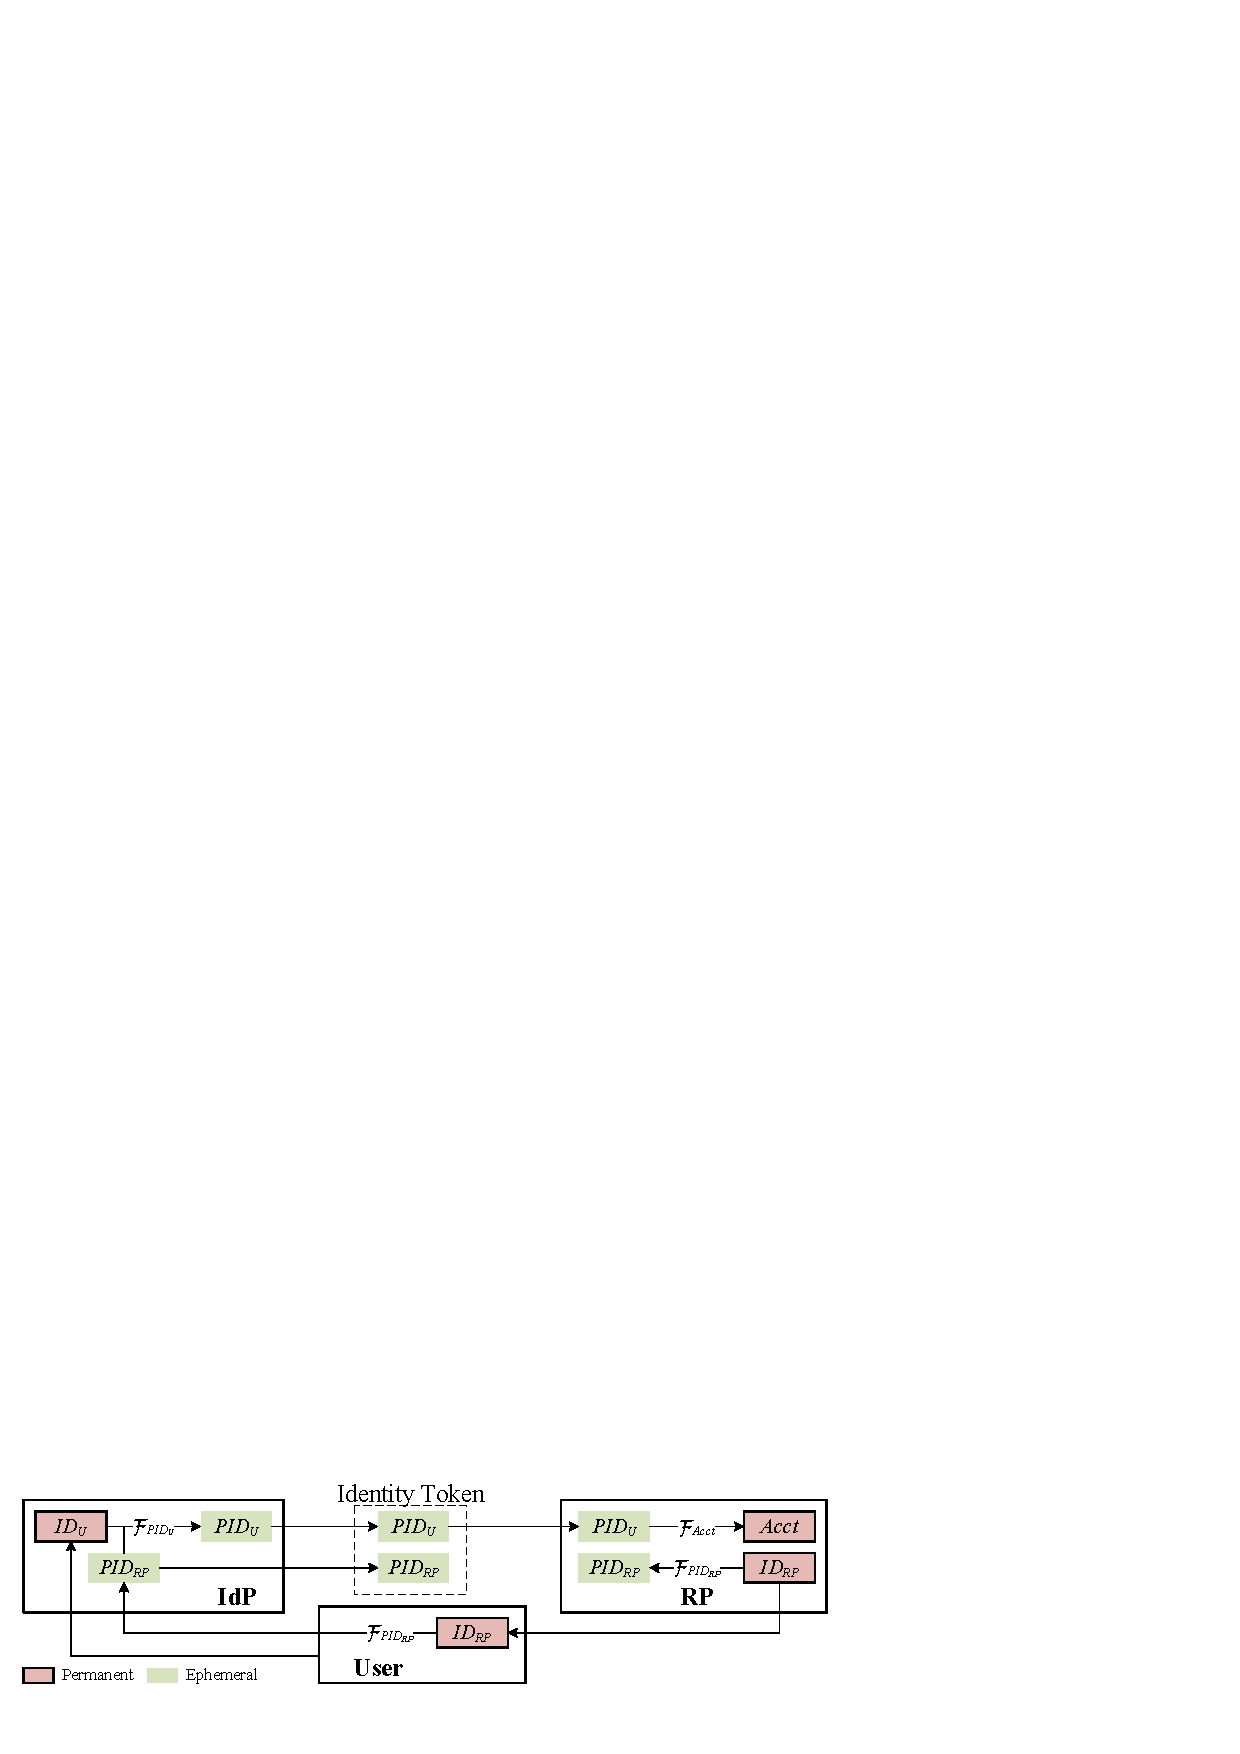
\includegraphics[width=1.00\linewidth]{fig/IDCorrelation.pdf}
  \caption{Identity transformations in UPPRESSO} %privacy-preserving SSO}
  \label{fig:IDCorrelation}
\end{figure}

In addition to the basic requirement of account uniqueness,
    user identification and RP designation ensure security of SSO services,
    while IdP untraceability and RP unlinkability protect user privacy
(see Section \ref{sec:analysis} for the formal proofs). 